\input sys/inputs.tex

\begin{document}

\bigheading{Kritické projekty}

% \info{task_name}{infile}{outfile}{points}{timelimit}{memlimit}
% leave this values, if you are not interested
\info{critical}{stdin}{stdout}{100}{600 ms}{32 MiB}

Stavba tunelu Blanka je rozdělená na $N$ menších projektů.
Hlavní architekt určil, které projekty je potrěbné dokončit před jinými projekty.
Jinými slovy, existují dvojice projektů $u$ a $v$, takové že projekt $u$ musí být dokončen dřív, než se začne pracovat na projektu $v$.
V takovém případě řekneme, že $u$ přímo předchází $v$.
Řekneme, že $u$ předchází $v$, pokud $u$ přímo předchází $v$, nebo existuje projekt $z$ takový, že $u$ přímo předchází $z$ a $z$ předchází $v$.

Projekt $u$ je považovaný za kritický, pokud pro každý projekt $v$ (jiný než $u$) platí, že buď $v$ předchází $u$ nebo $u$ předchází $v$.
Je známo, že tunel Blanka jde postavit, tzn. neexistuje žádný projekt $u$, který předchází sám sebe.

\heading{Úloha}

Napište program, který nalezne všechny kritické projekty.

\heading{Vstup}

První řádek vstupu obsahuje dvě celá čísla, $N$ a $M$.
$N$ ($1 \leq N \leq 100\,000$) je počet projektů a $M$ ($0 \leq M \leq 1\,000\,000$) je počet párů které se vzájemně přímo předchází.
Projekty jsou očíslované od $1$ do $N$.

Každý z následujících $M$ řádků obsahuje dvě celá čísla, $u$ a $v$ ($1 \leq u \neq v \leq N$), která znamenají, že projekt $u$ přímo předchází projekt $v$.

\smallskip
Pro $40 \%$ případů platí $N \leq 5\,000$ a $M \leq 30\,000$.

\heading{Výstup}

Na první řádek výstupu vypište počet kritických projektů. Na druhý řadek vypište mezerou oddělená číslá kritických projektů v roustoucím pořadí.

Pokud neexistují žádné kritické projekty, tak na výstup vypište pouze jeden řádek s číslem 0.

\heading{Příklady}

\sampleIN
7 9
1 3
2 3
3 4
3 5
4 6
5 6
1 7
3 7
7 4
\sampleOUT
2
3 6
\sampleCOMMENT

\sampleEND

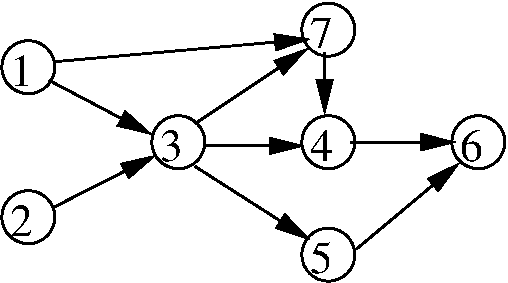
\includegraphics[height=4cm]{img/critical-fig.pdf}
\bigskip


\end{document}
